%Zarantonello Umberto 2021-04-22

\section{Esercizi}
\subsection{Settimana 1}
\subsubsection{Esercizio 1}
Si calcoli la velocità media di:
\begin{itemize}
\item Molecole d'aria a temperatura ambiente
\item Elettroni atomo idrogeno
\item Terra attorno al sole
\item Elettroni che escono da un vecchio tubo catodico
\end{itemize}

\paragraph{Risoluzione:}
\begin{itemize}
\item \textbf{Molecole d'aria}
supponiamo di essere a $20^oC$ corrispondenti a $293K$ si sfrutti la teoria cinetica dei gas
\begin{equation}
\frac{3}{2}K_BT=\frac{1}{2}m<v^2>
\end{equation}
Si approssimi l'aria come azoto $N_2$ la cui massa molecolare è $M_{N_2}=28$
si ottiene
\begin{equation}
\sqrt{<v^2>}=\sqrt{\frac{3K_BT}{m_{N_2}}}=\sqrt{\frac{3\times1,3\times10^{-23}293}{28\cdot 1,66\times10^{-27}kg}}=510\frac{m}{s}
\end{equation}
\item \textbf{Elettroni dell'idrogeno}
Ricordando la costante di Ridberg ovvero il potenziale di dissociazione dell'idrogeno, questa può essere considerata pari alla sua energia cinetica.
\begin{equation}
E=13.5eV=K_e\\
K=135\times10\cdot1,6\times10^{-19}J=2,1\times10^{-18}J=\frac{1}{2}m_ev^2
\end{equation}
conoscendo la massa dell'elettrone corrispondente a $m_e=9,1\times10^{-31}kg$ si ottiene che la velocità dell'elettrone sarà
\begin{equation}
v_e=\sqrt{\frac{2K_e}{m_e}}=2,1\times10^6\frac{m}{s}
\end{equation}
Si può notare che questa è una conferma che l'elettrone sia una particella non relativistica.
\end{itemize}
Si lasciano al lettore gli altri due punti.

\newpage
\subsubsection{Esercizio 2}
Si calcoli il numero di molecole nell'atmosfera.

\paragraph{Risoluzione:}
Si parte considerando la massa dell'atmosfera, che si può calcolare partendo dalla pressione atmosferica, corrispondente al dell'aria sopra un metro quadro.
\begin{equation}
p=10^5\frac{N}{m^2}\longrightarrow M=10^4\frac{kg}{m^2}
\end{equation}
Si consideri, ora la superficie della terra 
\begin{equation}
A_{terra}=4\pi R^2=12(6\times10^6m)^4=4\times10^14m^2
\end{equation}
Si può quindi trovare la massa dell'aria
\begin{equation}
M_{aria}=10^4\frac{kg}{m^2}4\times10^{14}m^2=4\times10^{18}kg
\end{equation}
Per calcolare il numero di molecole di aria, si consideri il pero molecolare di azoto e ossigeno
\begin{equation}
N_2=28\hspace{0,5cm}O_2=32
\end{equation}
Il che in media corrisponde ad un peso molecolare di $30$.
Una mole peserà dunque $30g$
\begin{equation}
M_{aria}=\frac{4\times10^21g}{30g/mol}=1,3\times10^{20}mol
\end{equation}
Il numero di molecole d'aria corrisponderà quindi alla massa in moli dell'aria moltiplicata per il numero di Avogadro $N_A=6\times10^{23}$
\begin{equation}
N_{aria}=M_{aria}\times N_A\simeq 10^41molecole
\end{equation}
Se si volesse poi sapere quante molecole di aria dell'ultimo respiro di Carlo Magno sono contenute nei nostri polmoni, si dovrebbe fare il rapporto fra la quantità di aria contenuta nei nostri polmoni e quella contenuta nell'atmosfera.
\begin{equation}
1mole (STP)=20L
\end{equation}
Una mole in condizioni standard corrisponde a 20 litri, la densità dell'aria corrisponderà quindi a 
\begin{equation}
30\frac{g}{mol}:20\frac{L}{mol}=1,5\frac{g}{L}\\
1L\sim 1g\sim 3\times 10^{22}molecole
\end{equation}
Qual è la frazione di molecole che noi respiriamo ad ogni respiro?
La massa dell'aria totale è pari a $4\times 10^21g$ e ogni respiro corrisponde ad un peso di circa $1g$, il che restituisce un rapporto di
\begin{equation}
0,25\times 10^{-21}
\end{equation}

\newpage
\subsubsection{Esercizio 3}
Una sorgente radioattiva di particelle $\alpha$ da 5,5 MeV viene collimata in modo tale che un fascetto quasi parallelo di 50000 particelle $\alpha$ al secondo colpiscano un sottile foglio di oro spesso 0,2$\mu m$.
In base alla legge di Rutherford, si determini il numero di particelle dflesse all'indietro ogni secondo (cioè ad angoli maggiori di $90^o$).
(\emph{Si trascuri il rinculo del nucleo di oro e si considerino: $\rho_{Au}=19300 kg/m^3$, $m_{Au}^{mol}=197 g/mol$, $Z_{Au}=79$}).

\paragraph{Risoluzione:}
\begin{equation}
dN=N_i\frac{d\sigma}{d\Omega}N_{t}d\Omega
\end{equation}
dove $N_i$ è il numero di particelle incidenti, $N_t$ è il numero di atomi per unità di superficie del bersaglio, $d\sigma/d\Omega$ è la sezione d'urto di Rutherford e $d\Omega$ è l'angolo solido di rivelazione.
\begin{equation}
\begin{split}
N_t&=\frac{n_atomi}{A}=\frac{m}{M_{Au}^{mol}}N_{Av}\frac{1}{A}\\
&=\frac{\rho_{Au}V}{M_{Au}^{mol}A}N_{Av}=\frac{\rho_{Au}}{M_{Au}^{mol}}N_{Au}t\\
&=\frac{\SI{19,3e3}{}\SI{6,02e23}{}\SI{0,6e-6}{}}{0,197}=\SI{1,18e22}{atm/m^2}
\end{split}
\end{equation}
Ci occupiamo ora della sezione d'urto di Rutherford interessandoci in questo caso solamente alle particelle diffuse indietro. 
L'integrale che dobbiamo fare in questo caso è
\begin{equation}
\begin{split}
\int_{indietro}N_i\frac{d\sigma}{d\Omega}N_td\Omega &=N_iN_t\int_{indietro}\frac{d\sigma}{d\Omega}2\pi \sin\theta d\theta\\
&=N_iN_t\int_{\frac{\pi}{2}}^{\pi}\frac{1}{(4\pi\varepsilon_0)^2}\frac{(z_1z_2e)^4}{16E^2}\frac{1}{\sin^4\frac{\theta}{2}}2\pi\sin\theta d\theta\\
&=2\pi N_iN_t\frac{1}{(4\pi\varepsilon_0)^2}\frac{(z_1z_2e)^4}{16E^2}\int_{\frac{\pi}{2}}^{\pi}\frac{\sin\theta}{\sin^4\frac{\theta}{2}}d\theta
\end{split}
\end{equation}
Si risolve ora l'integrale sapendo che $\sin\theta=2\sin\frac{\theta}{2}\cos\frac{\theta}{2}$ 
\begin{equation}
\begin{split}
\int_{\frac{\pi}{2}}^{\pi}\frac{2\sin\frac{\theta}{2}\cos\frac{\theta}{2}}{\sin^4\frac{\theta}{2}}d\theta&=2\int_{\frac{\pi}{2}}^{\pi}\frac{\cos\frac{\theta}{2}}{\sin^3\frac{\theta}{2}}d\theta\\
&=\biggl[\frac{2}{\sin^2\frac{\theta}{2}}\biggl(-\frac{1}{2}\biggl)\biggl]^\pi_{\frac{\pi}{2}}=2
\end{split}
\end{equation}
Calcoliamo quindi il fattore moltiplicativo dell'integrale
\begin{equation}
\left(\frac{e^2}{4\pi\varepsilon_0}\right)^2=\left(\frac{e^2\hbar c}{4\pi\varepsilon_0 \hbar c}\right)^2=(\alpha \hbar c)^2=(\SI{1,44}{MeV fm})^2
\end{equation}
Si ottiene quindi
\begin{equation}
\begin{split}
&=4\pi N_iN_t(\alpha \hbar c)^2\frac{z_1z_2}{16E^2}=\\
&=1256\cdot\SI{5e4}{1/s}\cdot\SI{1,18e22}{1/m^2}\cdot\frac{\SI{2,07}{MeV^2 fm^2}(2\times 79)}{16\cdot30\cdot25 MeV^2}=\\
&=0,8part./s=2880part/h
\end{split}
\end{equation}

\newpage
\subsubsection{Esercizio 4}
si calcoli l'energia contenuta in un $kg$ di benzina, approssimando la benzina come $CH_2$.
\paragraph{Risoluzione:}
Si può stimare che per ogni legame chimico l'energia sia pari a $E=1,5eV$ (\'E una stima molto approssimata).
Si considerino le masse atomiche:

Il carbonio ha massa atomica $C=12$, mentre l'idrogeno $H=1$, il che riconduce ad una massa totale pari a $CH_2=14$.

In un $Kg$ di benzina si ha
\begin{equation}
N_{moli} =\frac{1Kg}{1,4\times 10^{-2}Kg/mol}=70mol
\end{equation}
Per ogni molecola di $CH_2$ avrò due reazioni
\begin{equation}
C+O_2\longrightarrow CO_2\\
H_2+O\longrightarrow H_2O
\end{equation}
Corrispondente ad un'energia totale rilasciata di $3eV$.

Qual'è la densità energetica della benzina?
\begin{equation}
D=70\frac{mol}{Kg}\cdot 6\times 10^{23}\frac{reazioni}{mol}\frac{3eV}{mol}\cdot \frac{1}{1,6\times 10^{-19}eV/J}=2\times 10^7\frac{J}{Kg}
\end{equation}
Questo valore è approssimativo ma si discosta solamente di un fattore 2 dal valore reale, il che ci f intuire che comunque si tratta di un buon calcolo (che il bravo fisico deve essere in grado di effettuare).

Qual è poi la potenza trasferita in un pieno?

Supponiamo che un serbatoio di un'auto di $80L$. La densità della benzina è più bassa di quella dell'acqua. 
La densità di energia per litro corrisponde a $3\times10^7J/L$
\begin{equation}
80L\cdot 3\times10^7\frac{J}{L}=2\times10^9J
\end{equation}
In 3 minuti (tempo di un pieno) l'energia trasferita corrisponde a 
\begin{equation}
P=\frac{E}{\Delta t}=\frac{2\times10^9J}{180s}=10MW
\end{equation}
Impressionante!

\newpage
\subsubsection{Esercizio 6}
Produzione energetica
\begin{itemize}
\item Si stimi il fabbisogno energetico annuo di combustibile di una centrale a carbone da 1 GW.
\item Si stimi il numero di molecole di $CO_2$ iniettate nell'aria dalla centrale.
\item Si stimi la potenza prodotta da una turbina eolica.
\item Si stimi il fabbisogno annuo di uranio di una centrale nucleare da 1 GW.
\end{itemize}

\paragraph{Risoluzione:}
Similmente a come si è ottenuto il contenuto energetico della benzina è possibile ottenere quella del carbone. 
La densità energetica del carbone sarà all'incirca di $1,5 eV$ per legame, bisogna quindi cercare il numero di legami della molecola di carbone.
Consideriamo che la massa sia composta solo da carbonio 12 $^{12}_6C$.
1 mole di $^{12}_6C$ avrà massa pari a $M_C=\SI{1,2e-2}{kg}$, un $kg$ di Carbone conterrà quindi
\begin{equation}
\frac{1kg}{\SI{1,2e-2}{kq/mol}}=80 mol
\end{equation}
L'energia al $kg$ del carbone corrisponde quindi a 
\begin{equation}
D_C=\frac{1,5eV}{atomo}\SI{6e-23}{}\frac{atomi}{mol}80mol\cdot 1,6\times10^{-19}\frac{j}{eV}=\SI{e7}{j/kg}
\end{equation}
Avendo una centrale da 1GW, e supponendo che l'efficienza sia circa del $30\%$ si ha che l'energia termica corrisponde a 3GW.
L'energia termica richiesta corrisponderà dunque a 
\begin{equation}
E_{anno}=3\times10^9\frac{j}{s}  \pi\times 10^7\frac{s}{anno}=10^7j/anno
\end{equation}
La massa di carbone richiesta sarà dunque
\begin{equation}
M_C=\frac{E_{anno}}{D_c}=\frac{10^{17} j/anno}{2\times 10^7 j/kg}=\SI{5e9}{kg/anno}
\end{equation}
(è stato usato un valore reale di densità energetica e non quello approssimato ottenuto sopra).
C'è bisogno di 5 milioni di tonnellate di carbone corrispondenti a 500 treni da 100 vagoni, una quantità che richiede una certa struttura per la gestione dei rifornimenti.

Analizziamo ora una centrale nucleare da 1 GW.
Per ogni fissione si ha una reazione del tipo
\begin{equation}
_{92}^{235}U\longrightarrow X+Y
\end{equation}
che produce un'energia di 200 MeV corrispondente ad un fatto di $10^8$ rispetto all'energia di legame chimica.
Il conto poi sarà identico alle centrali a carbone in quanto il funzionamento è il medesimo.
\begin{equation}
1GW_{ele}=1GW_{th}\longrightarrow E_{anno}=10^{17}\frac{j}{anno}
\end{equation}
Bisogna calcolare la densità energetica dell'uranio.
\begin{equation}
D_{^{235}U}=2\times10^8\frac{eV}{nucleo}\times 6\times10^{23}\frac{atm}{mol}\times2\times10^{-19}\frac{j}{eV}\times4\frac{mol}{kg}=\SI{8e13}{j/kg}
\end{equation}
In natura l'uranio 235, materiale fissile, è presente allo $0,72\%$ nell'uranio. 
Nelle centrali si sfrutta l'uranio arricchito con una densità del $5\%$ di materia fissile.
La densità energetica effettiva sarà quindi di 
\begin{equation}
D_U=0,05\times\SI{8e13}{j}=E_{eff}=\SI{4e12}{j/kg}
\end{equation}
La massa di Uranio richiesta sarà quindi di 
\begin{equation}
M=\frac{10^{17}j/anno}{4\times10^{12}j/kg}=\SI{2e4}{kg/anno}
\end{equation}
La densità dell'uranio è di circa $20\times10^3 kg/m^3$, il che vuol dire che ci basta $1 m^3/anno$ di Uranio.


\section{Tavola periodica degli elementi}
\begin{figure}[h]
\centering
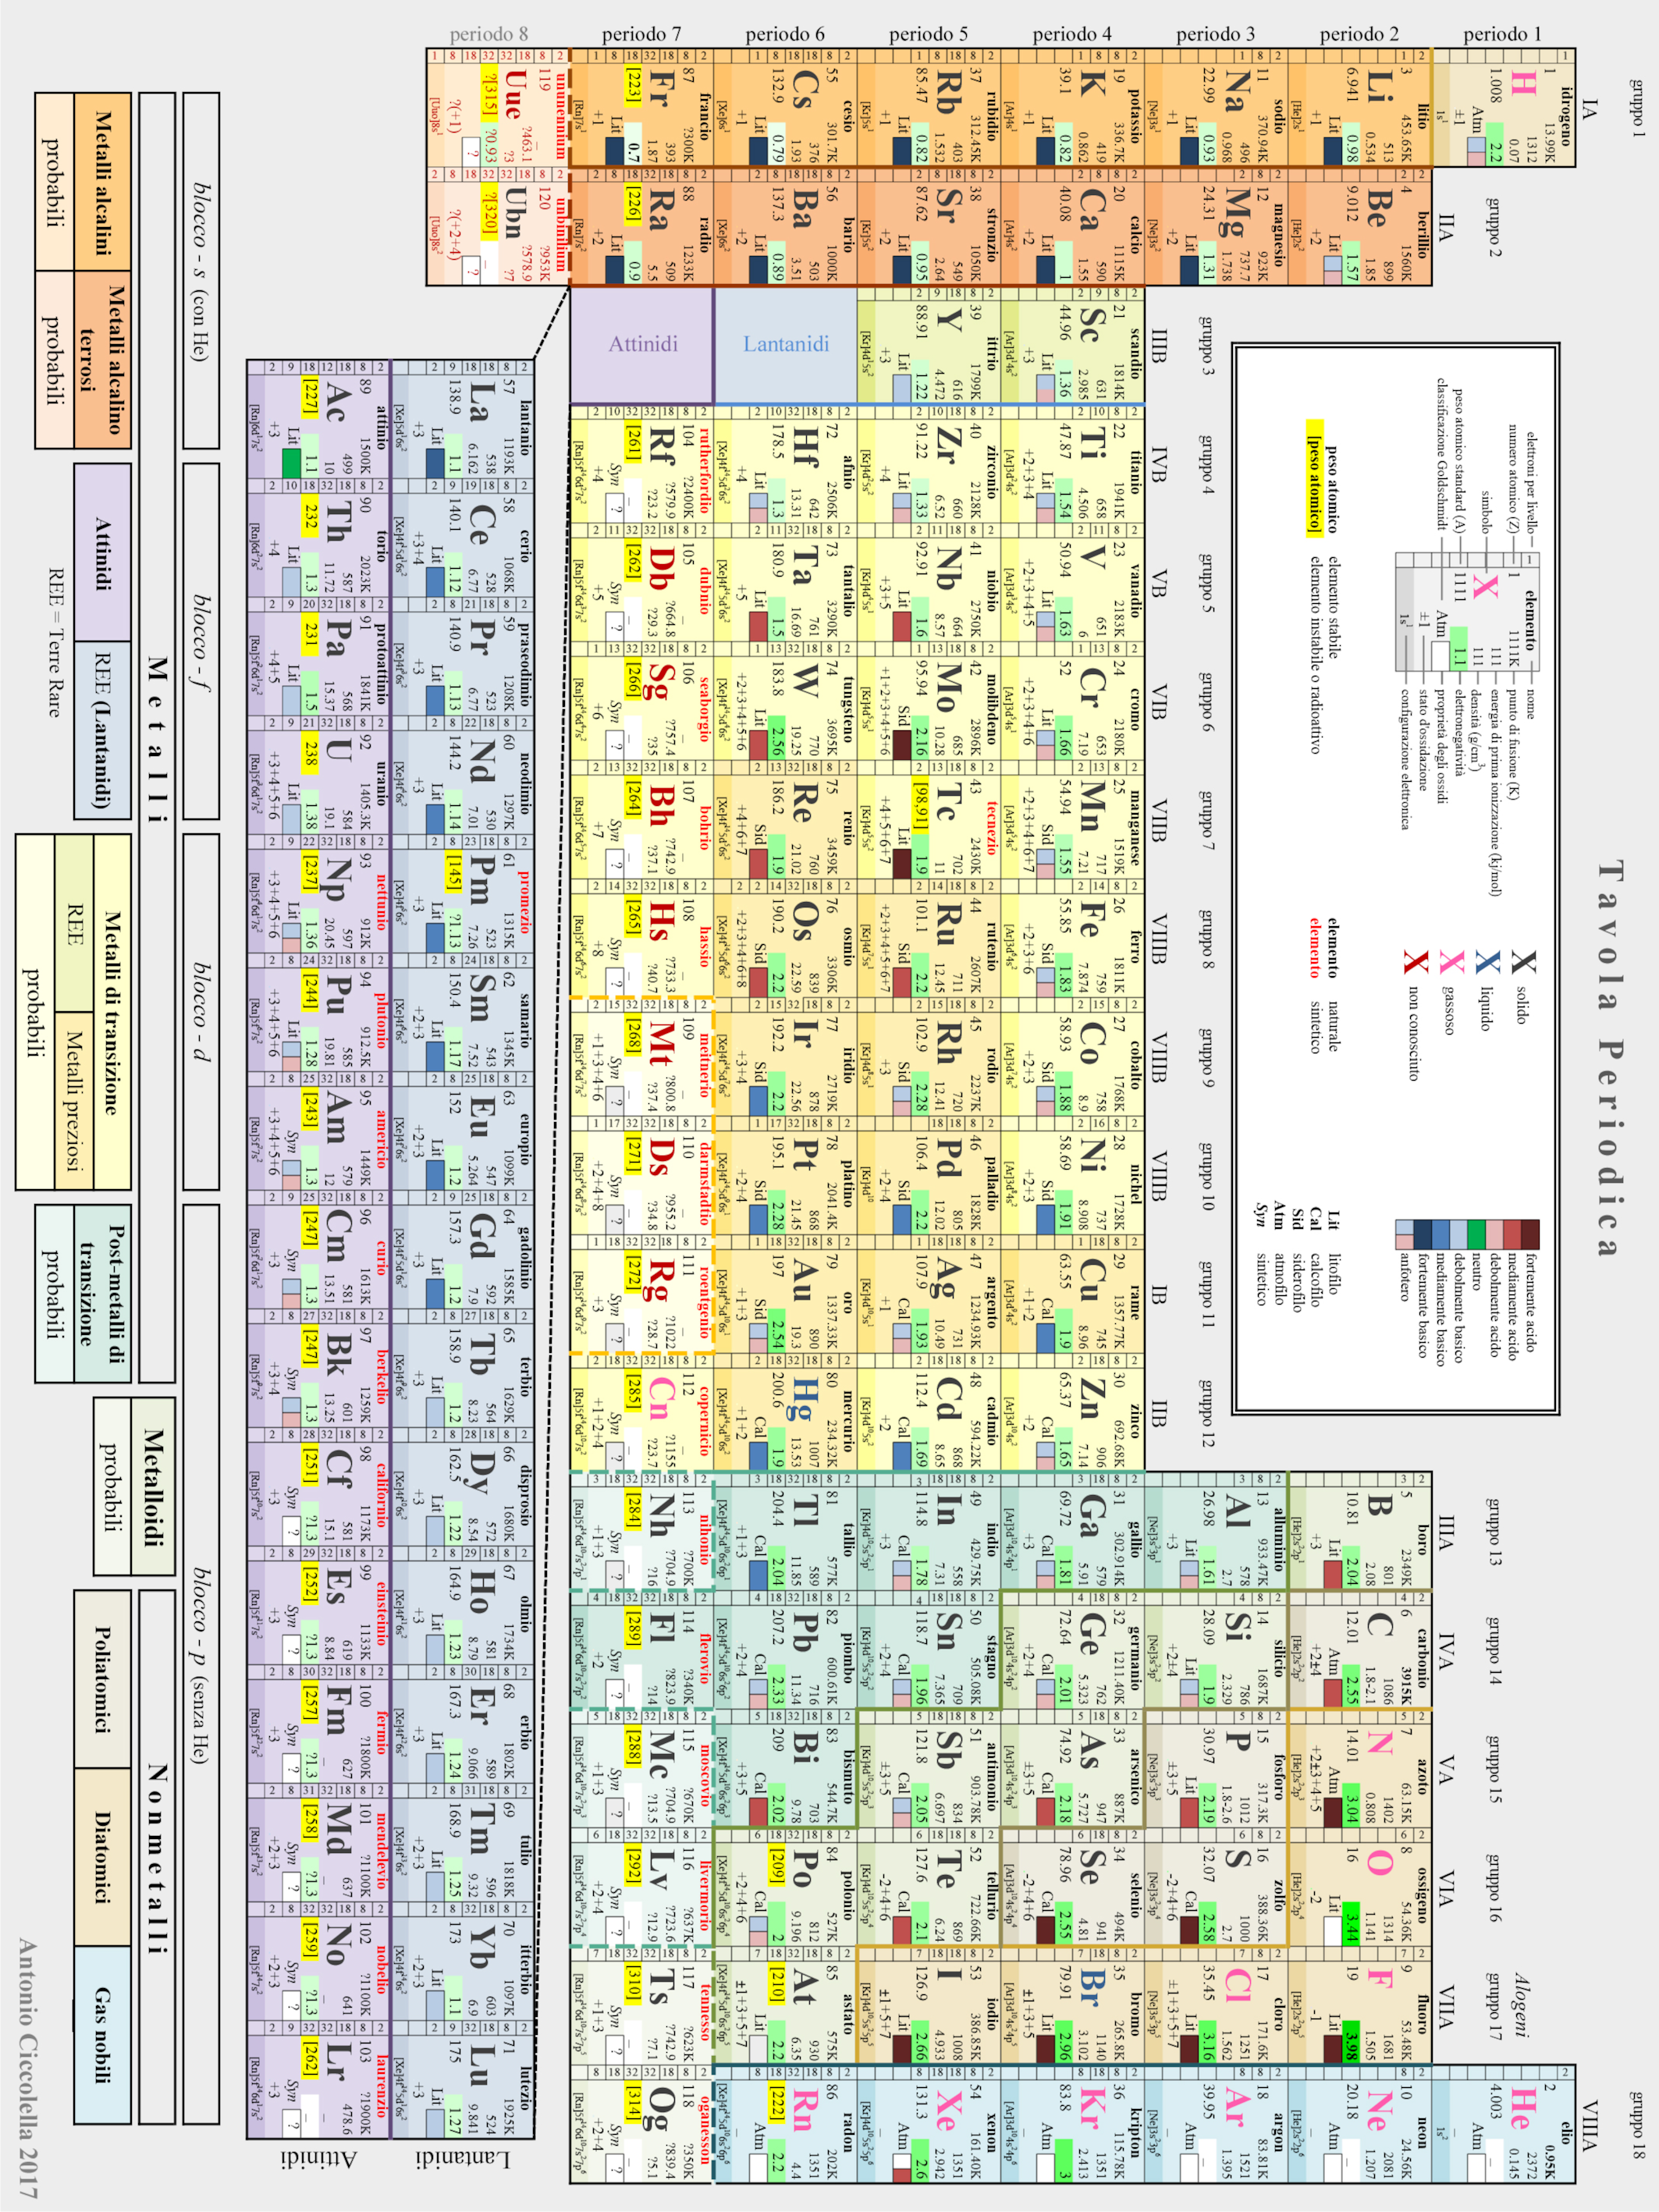
\includegraphics[scale=0.7]{/Tavola_periodica_2013}
\caption{Tavola periodica degli elementi}
\end{figure}
